In this section, the shape of some key distributions are compared for for the two signal processes, namely $gu \to tt \bar{u}$ and $uu \to tt$, 
and the two main backgrounds relevant for the $tt+X$ final state, namely $t\bar{t}$ (via charge mis-reconstruction) and $t\bar{t} + V$. The 
distributions are obtained at the truth hadronic level, without any detector effects. The objects are selected using criteria close from those
used in the Run 1 analysis.


\begin{figure}[!h!tpd]
  \centering
  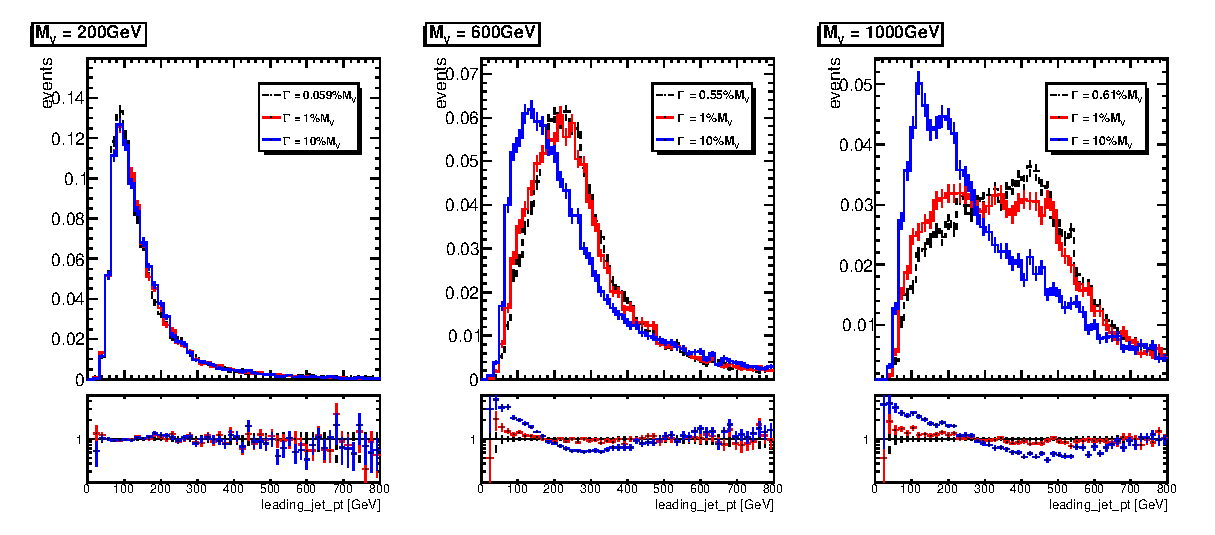
\includegraphics[width=0.48\textwidth]{appendix/appendixC/leading_jet_pt.eps}
  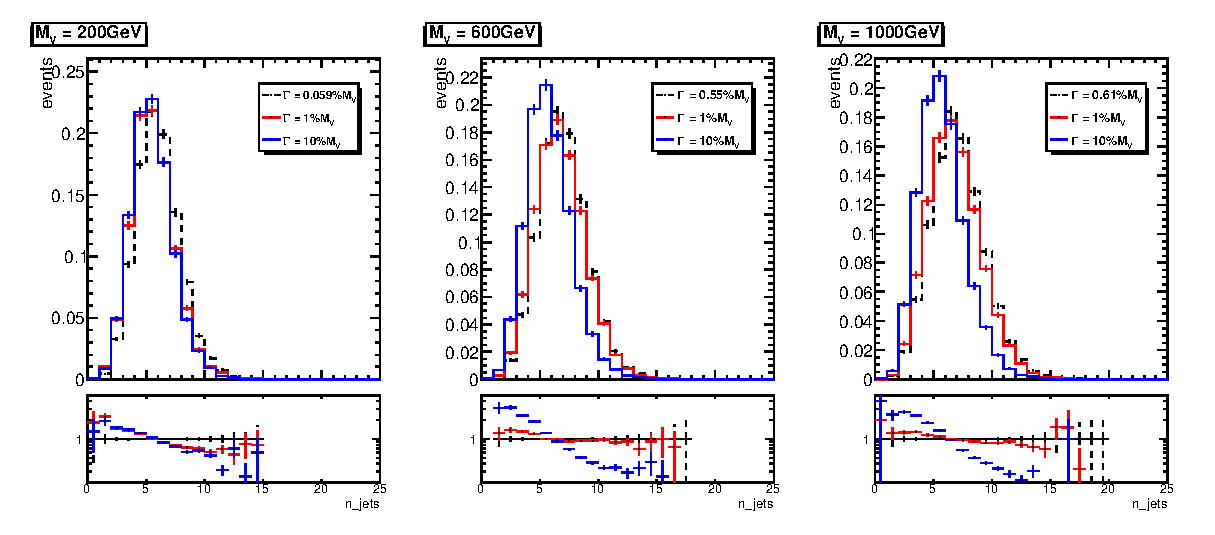
\includegraphics[width=0.48\textwidth]{appendix/appendixC/n_jets.eps}
  \caption{
      Distribution of the leading jet $p_T$ for signals ($m_V=600~\GeV{}$, $\Gamma_V$ computed in MadGraph) and backgrounds at the (hadronic) thruth level.
  }   
  \label{fig:appB:Vmass}
\end{figure}


%\begin{figure}[!h!tpd]
%  \centering
%  \caption{
%      Distribution of the jet multiplicity for all processes leading to $tt+X$
%      for $m_V = \{200, 600, 1000\}~\GeV{}$ (from left to right) and for three different
%      visible decay width (computed from Madgraph directly, $1\%$ and $10\%$).
%  }   
%  \label{fig:appB:Vmass}
%\end{figure}


\begin{figure}[!h!tpd]
  \centering
  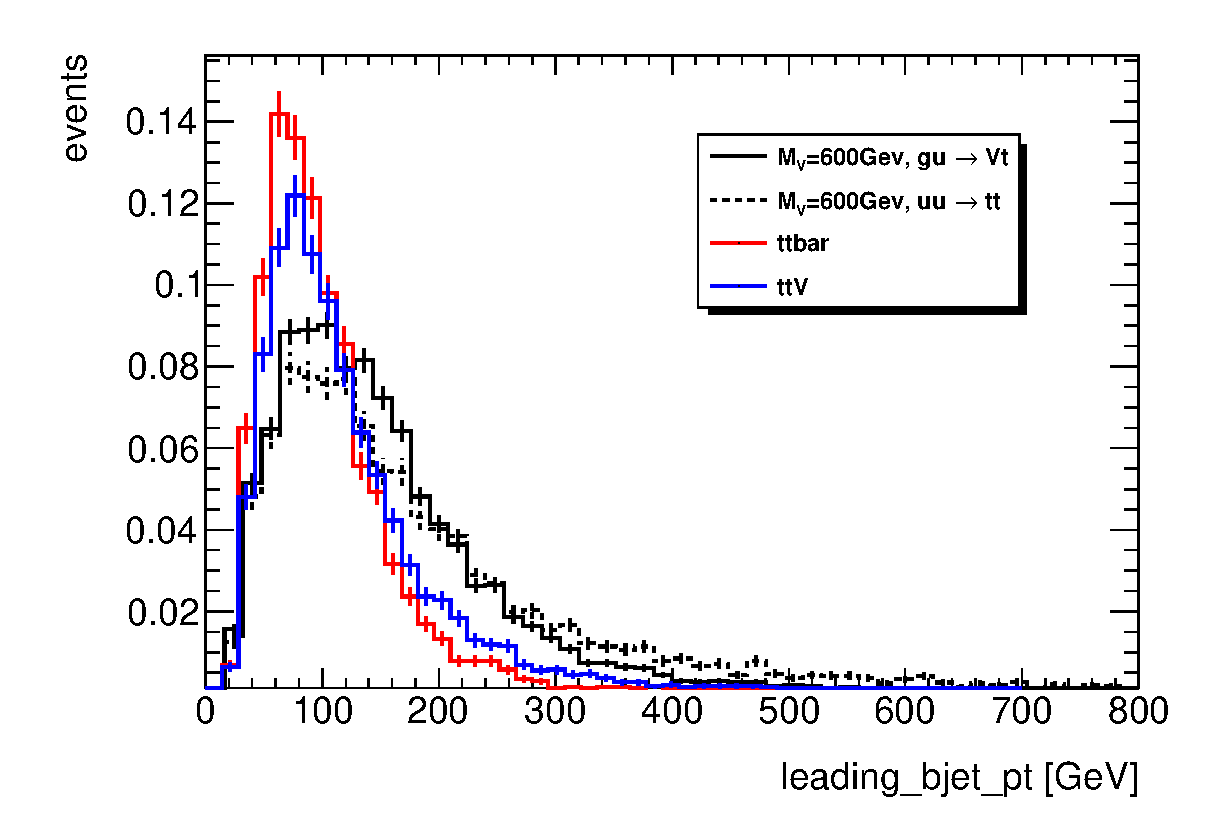
\includegraphics[width=0.48\textwidth]{appendix/appendixC/leading_bjet_pt.eps}
  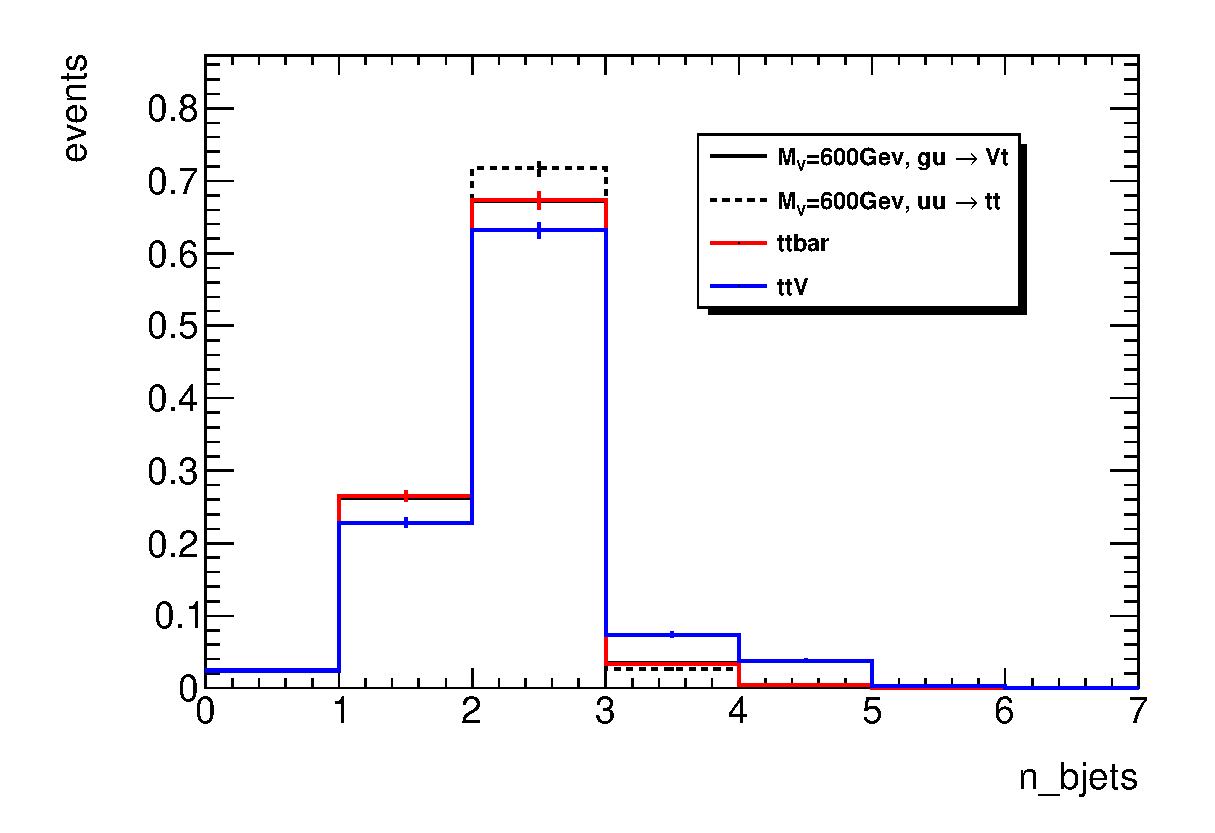
\includegraphics[width=0.48\textwidth]{appendix/appendixC/n_bjets.eps}
  \caption{
      Distribution of the leading jet $p_T$ for signals ($m_V=600~\GeV{}$, $\Gamma_V$ computed in MadGraph) and backgrounds at the (hadronic) thruth level.
  }   
  \label{fig:appB:Vmass}
\end{figure}


%\begin{figure}[!h!tpd]
%  \centering
%
%  \caption{
%      Distribution of the jet multiplicity for all processes leading to $tt+X$
%      for $m_V = \{200, 600, 1000\}~\GeV{}$ (from left to right) and for three different
%      visible decay width (computed from Madgraph directly, $1\%$ and $10\%$).
%  }   
%  \label{fig:appB:Vmass}
%\end{figure}


\begin{figure}[!h!tpd]
  \centering
  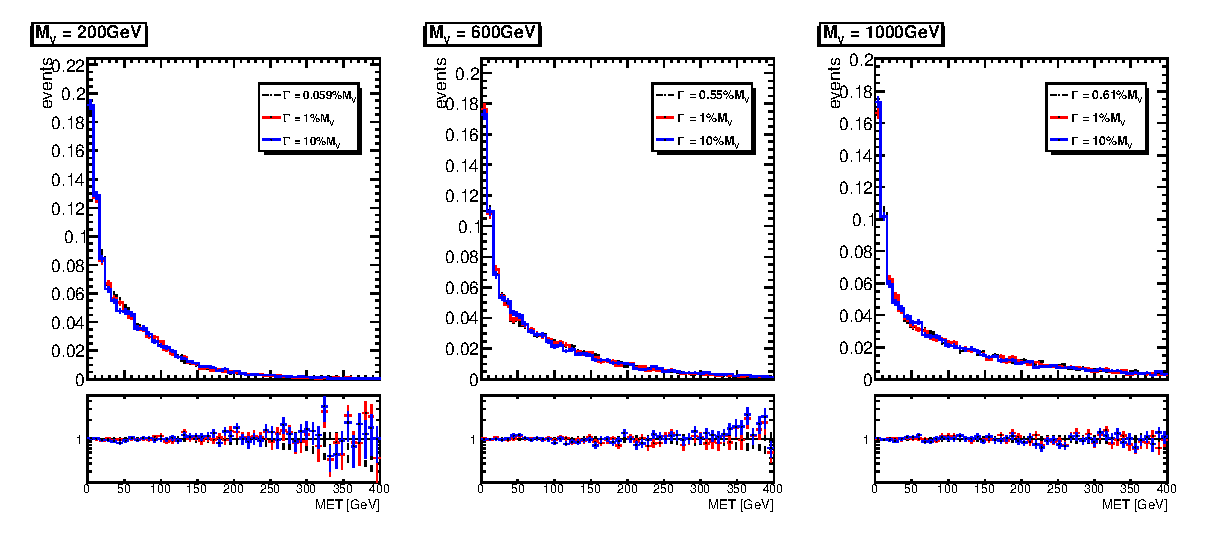
\includegraphics[width=0.48\textwidth]{appendix/appendixC/MET.eps}
  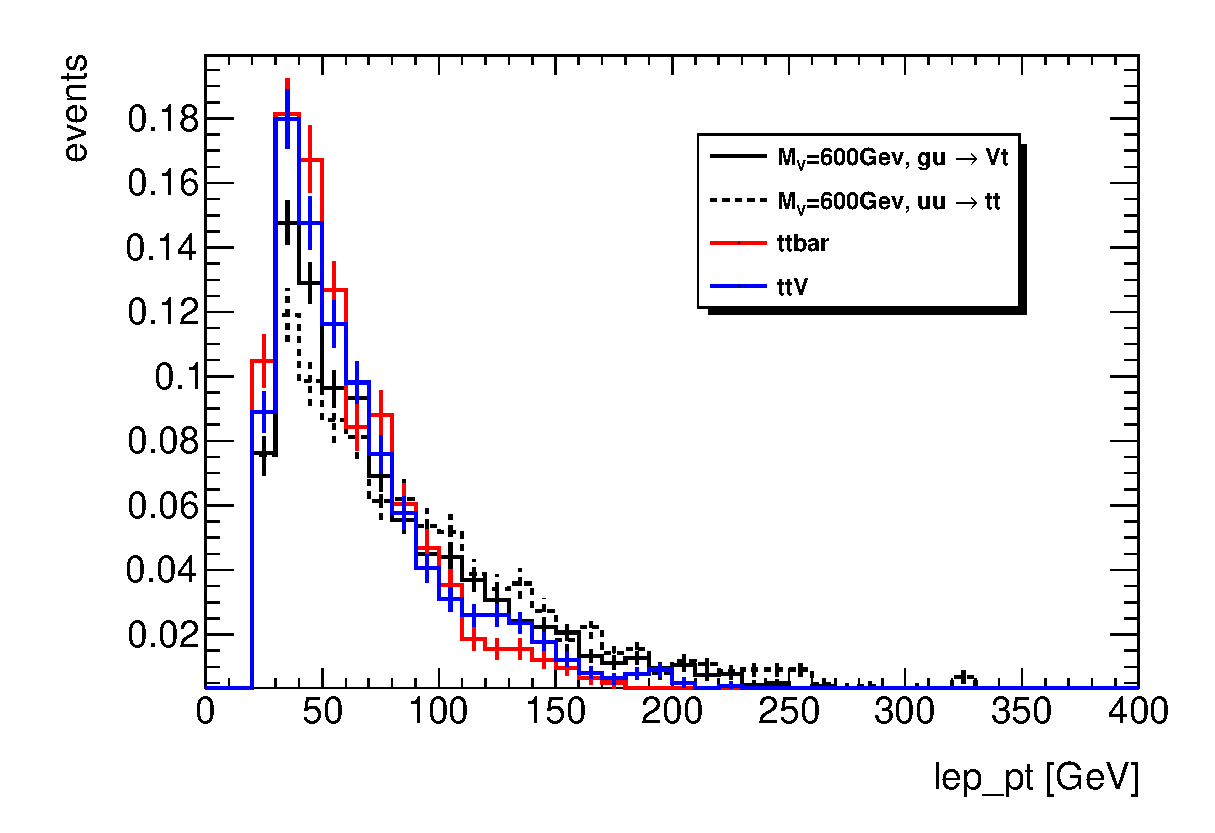
\includegraphics[width=0.48\textwidth]{appendix/appendixC/lep_pt.eps} 
 \caption{
      Distribution of the $\met$ for signals ($m_V=600~\GeV{}$, $\Gamma_V$ computed in MadGraph) and backgrounds at the (hadronic) thruth level.
  }   
  \label{fig:appB:Vmass}
\end{figure}

%\begin{figure}[!h!tpd]
%  \centering
% 
%  \caption{
%      Distribution of the lepton $p_T$ for all processes leading to $tt+X$
%      for $m_V = \{200, 600, 1000\}~\GeV{}$ (from left to right) and for three different
%      visible decay width (computed from Madgraph directly, $1\%$ and $10\%$).
%  }   
%  \label{fig:appB:Vmass}
%\end{figure}


\begin{figure}[!h!tpd]
  \centering
  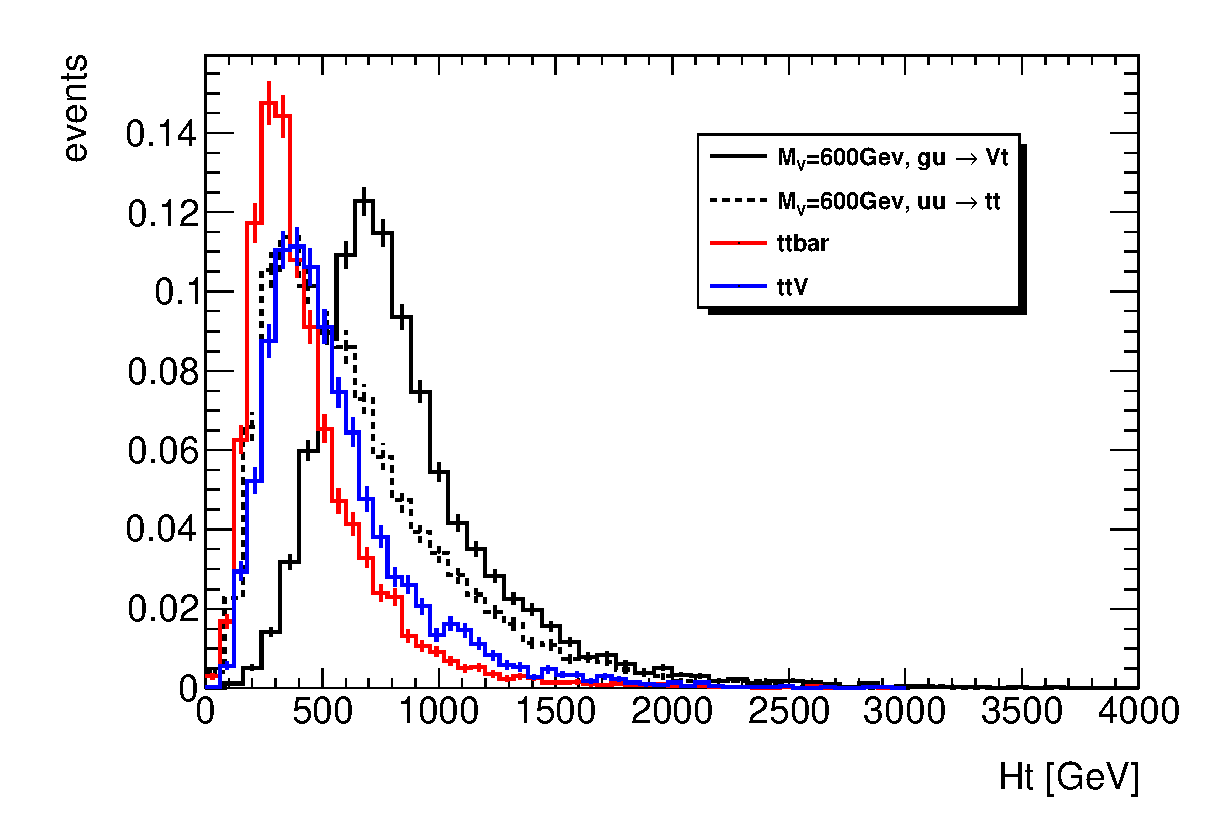
\includegraphics[width=0.65\textwidth]{appendix/appendixC/Ht.eps}
  \caption{
      Distribution of the $p_T$ scalar sum ($H_T$) for signals ($m_V=600~\GeV{}$, $\Gamma_V$ computed in MadGraph) and backgrounds at the (hadronic) thruth level.
  }   
  \label{fig:appB:HT}
\end{figure}

